\documentclass[conference]{IEEEtran}
\usepackage[noadjust]{cite}
\usepackage{amsmath}
\usepackage{algorithm}
\usepackage[noend]{algpseudocode}
\usepackage{graphicx}
\usepackage{subcaption} 
\usepackage{verbatimbox}
\usepackage{multirow}
\usepackage{pbox}
\usepackage{tabularx}
\usepackage{adjustbox}
\usepackage{rotating}
\usepackage{epstopdf}
\usepackage[justification=centering]{caption}% or e.g. [format=hang]


\hyphenation{op-tical net-works semi-conduc-tor}    

\title{User Authentication\\via Mouse Movements}

\begin{document}
\maketitle


\begin{abstract}
The abstract goes here.
\end{abstract}
\IEEEpeerreviewmaketitle

\section{Introduction}


\begin{figure}[h!]
  \includegraphics[width=1\linewidth]{Overview.pdf}
\caption{An overview of continuous verification with mouse movements. In the training phase a user creates a profile based on their mouse movements (The average and standard deviation of each mouse feature). The profile is used to represent a user in the verification phase where features from live mouse movements can be verified against the profile in order to determine if the live mouse movements came from the user who created the profile. If the verifier determines that the live mouse movements are illegitimate an action can be taken. ( e.g. logging the user out, creating a log of the incident, etc.)}
\end{figure}

\section{Data Collection}
We wanted our data set to include movements that were natural to best simulate day to day actions a user would perform on the computer in order to have a more relevant set of data to what our authenticator would see in a practical environment. To do this we asked a class of students to record themselves and two other friends or family members. The students were told to instruct whomever was being recorded to go about any activity on the computer they normally would for an hour period.  
	In order to log the mouse activity of users we created a simple mouse logger.  The logger was a small piece of software that ran on the windows operating system. The logger, when run on a machine, logged the position of the cursor using the windows method GetCursorPos(), the state of the left and right mouse buttons (up or down), and a timestamp every 15.6ms. 15.6ms being the default timer resolution that windows supports. The resulting log was then placed into a text file. 
We then screened the samples and removed samples with very few (0 – 10) movements and samples that weren't an hour long. Post-screening we had 25 valid user samples.  Our samples consisted of university students and their friends and family collected from late November to early December 2014.


\bgroup
\def\arraystretch{1.5}
\addvbuffer[12pt 8pt]{\begin{tabular}{l*{6}{c}r}
\textbf{Type}              &\textbf{ Maximum} & \textbf{Minimum} & \textbf{Average} \\
\hline
Left Clicks	& 716 & 37 & 547.84 \\
Right Clicks	& 690 & 0 & 122.8 \\
Double Clicks	& 1282 & 1 & 181.64 \\

\end{tabular}}
\egroup
\captionof{table}{Overview of the samples collected}


\section{Feature Extraction}
	We defined a mouse movement as a period of cursor movement followed by a click. This isn't to say that a click without any movement prior is not considered a mouse movement. It would be a mouse movement with no speed, acceleration, or jerk. If the cursor sustains no action for a period of 500ms or longer we classify that period as a pause to allow for periods where the user is not concentrating on moving the mouse or not moving it with conscious effort.

\bgroup
\def\arraystretch{1.5}
\begin{table*}
\begin{tabular}{m{.25\textwidth} | m{.75\textwidth}  }
  
 \textbf{ Feature}	&	\textbf{Description}\\
 \hline
 Single Left Click Length	&	\multirow{2}{*}{\pbox{20cm}{The length of a click from the first record the mouse button is found to be \\ down to the first record the mouse button is found to be up.}}\\
\cline{1-1}
 Single Right Click Length	&	\\
\hline
 Double Click Length	&	\pbox{20cm}{Split into 4 sub-features: Total Length and intervals 1,2, and 3.\\
Total length: The time between the first record the mouse is found to be down and the first record the mouse\\ is found to be up after the second click.\\
Interval 1: The first single left click length in a double click.\\
Interval 2: The time between the first record of the left mouse button being found up after the first click to the\\ first record of the left mouse button being found down for the second left click.\\
Interval 3: The second single left click length in a double click.}\\
\hline
 Speed			&	Distance the cursor travelled divided by the total time of the movement up until the click.\\
\hline
Acceleration			&	Change in Speed over time\\
\hline
Jerk				&	Change in Acceleration over time\\

\end{tabular}
\caption{Descriptions of the features used}
\end{table*}
\egroup




\section{Methodology}


\subsection{Outlier Filtering}
For our setup we first went through each of the user samples and extracted each of the features, as defined above, from each mouse movement. To remove rare cases of mouse movements where the user provides a mouse movement far from the mean we implemented an outlier removal scheme. We define a mouse feature to be an outlier if it is more eccentric than 66% of the population of the same mouse features for a single user. For example, if we are looking to find if a particular mouse feature M is an outlier:

\begin{algorithm}
\caption{Determines if a single feature F is an outlier from the rest of the population of its own kind}\label{euclid}
\begin{algorithmic}[1]
\Procedure{IsAnOutlier}{$F$}
\State $\textit{count} \gets 0$
	\For{\textbf{each} $feature \textrm{ in } featurePopulation$}
			\If{$ |F - feature| > R$}
				\State $count \gets count + 1$
			\EndIf
	\EndFor
	\If{$count \div featurePopulation_{size} \ge .33$}
		\State \Return{\texttt{True}}
	\Else
		\State \Return{\texttt{False}}
	\EndIf
\EndProcedure
\end{algorithmic}
\end{algorithm}

We defined the variable R, for each mouse feature, a number large enough to include most of the population while small enough to remove the noise from the data. We found optimal values for our R values after extensive experimentation we will describe later on.


\begin{figure}[t]
  \includegraphics[width=1\linewidth]{clickDiag}
  \caption{A visual representation of the click features. Dashes representing no button activity, dots representing periods where the mouse button is down, and vertical bars representing the first record that the mouse button has changed state.}
\end{figure}

\subsection{Verification}
	To authenticate a user based on their mouse movements we analyze six mouse features over the course of a sample. Our method is a simplistic user-authentication model. We create a profile based on a user's past behavior then test further samples against that profile to determine if the sample we test with is close enough to the previous profile to be considered the same user.  
We then split the edited list of features into a testing set and a training set. For each file we create user profiles based on half of the user's sample (about 50 mouse movements on average for our samples). The profiles being simply the averages and standard deviations of each of the mouse features. The mouse movements from the sample that we did not use for the profile go into the user's testing set.
Using a simple classification scoring method we can see how well a user profile and a testing set of data match up. For our entire set of data we took every user profile and tested each against every testing set. Our custom testing method generated a score for each test between 0 and 1. 1 being a perfect match and 0 being a perfect mismatch.
We tested by comparing each of the mouse movements in a testing set against the users profile. If the features in the mouse movement are within m standard deviations of the corresponding means in the user profile then the test gets a point. The total amount of points accrued is divided by the total amount of mouse movements in the file to generate the score.
	


\section{Experimental Setup}
We had a few parameters where it wasn’t immediately apparent how to set. For the R variables we needed values that can discriminate mouse feature values that are too eccentric while keeping as much unique data as possible. To solve this we ran a script that ran the tests and found the EER over an array of values for each parameter to determine the optimal values where the EER is at its lowest. We found that an M value of 1.9, a Single Click R of 15, and a Double Click R of 175 to produce the lowest EER for our set of data.

\bgroup
\def\arraystretch{1.5}
\addvbuffer[12pt 8pt]{\begin{tabular}{ l| l}
\textbf{Parameter}              &\textbf{ Values Tested} \\
\hline
Single Click R		& 15 20 25 30 25  \\
Double Click R	& 175 180 185 190 195\\
M Values		& 0.7 1 1.3 1.6 1.9 2.2 2.3\\
\end{tabular}}
\egroup
\captionof{table}{The values used for our parameters for testing.}



\section{Experimental Results \& Analysis}
To calculate the results of our experiment we took each users profile and tested that against every other set of testing data. This values in this generated confusion matrix are then used to calculate the false rejection rate and false acceptance rate. After finding the best settings for our parameters we obtained 6.7\% equal error rate. 

\bgroup
\def\arraystretch{1.5}
\addvbuffer[12pt 8pt]{\begin{tabular}{ c  l | l l l l l }

         \multirow{11}{*}{\begin{sideways} \textbf{ M-Values}\end{sideways}} & \multicolumn{6}{c}{\textbf{R-Values}} \\


       && \textbf{175}  &  \textbf{180}  &  \textbf{185}  &  \textbf{190}  &  \textbf{195} \\
\cline{2-7}
 
   & \textbf{.7}	&14.86\%	&10.53\%	&9.33\%	&9.33\%	&8.99\%\\
   &\textbf{1}	&30.02\%	&24.23\%	&24.23\%	&27.37\%	&24.00\%\\
  &\textbf{1.3}	&14.46\%	&13.90\%	&10.40\%	&13.56\%	&13.33\%\\
   &\textbf{1.6}	&11.35\%	&10.40\%	&10.40\%	&10.59\%	&11.81\%\\
   &\textbf{1.9}	&13.35\%	&12.00\%	&12.00\%	&11.81\%	&11.36\%\\
   &\textbf{2.2}	&13.36\%	&6.77\%	&6.70\%	&6.72\%	&6.88\%\\
  & \textbf{2.5}	&7.71\%	&8.00\%	&8.00\%	&7.89\%	&7.50\%\\
\end{tabular}}
\egroup
\captionof{table}{The EER rates found across multiple parameter values. Each column is a separate double click R-value while each row is a separate M-value. The entire table is tested with one single click R-value set to 20ms.}


\begin{figure*}[t!]
\begin{subfigure}{.5\textwidth}
  \centering
  \includegraphics[width=.8\linewidth]{Optimal}
  \caption{Optimal Settings\\Single Click R = 15ms Double Click R = 175ms\\M-Value = 2.2}
  \label{fig:sfig1}
\end{subfigure}%
\begin{subfigure}{.5\textwidth}
  \centering
  \includegraphics[width=.8\linewidth]{7M}
  \caption{Single Click R = 35ms Double Click R = 195ms\\M-Value = 0.7}
  \label{fig:sfig2}
\end{subfigure}
\begin{subfigure}{.5\textwidth}
  \centering
  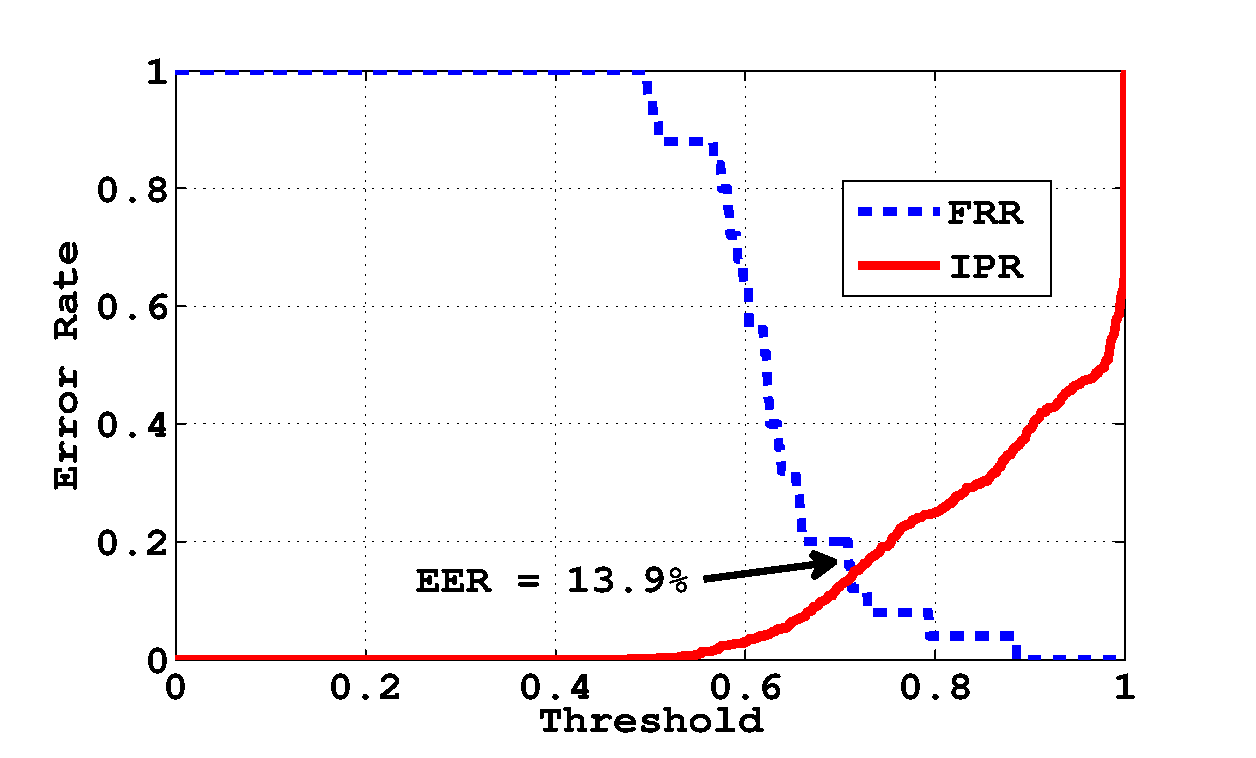
\includegraphics[width=.8\linewidth]{M1}
  \caption{Single Click R = 20ms Double Click R = 180ms\\M-Value = 1}
  \label{fig:sfig3}
\end{subfigure}%
\begin{subfigure}{.5\textwidth}
  \centering
  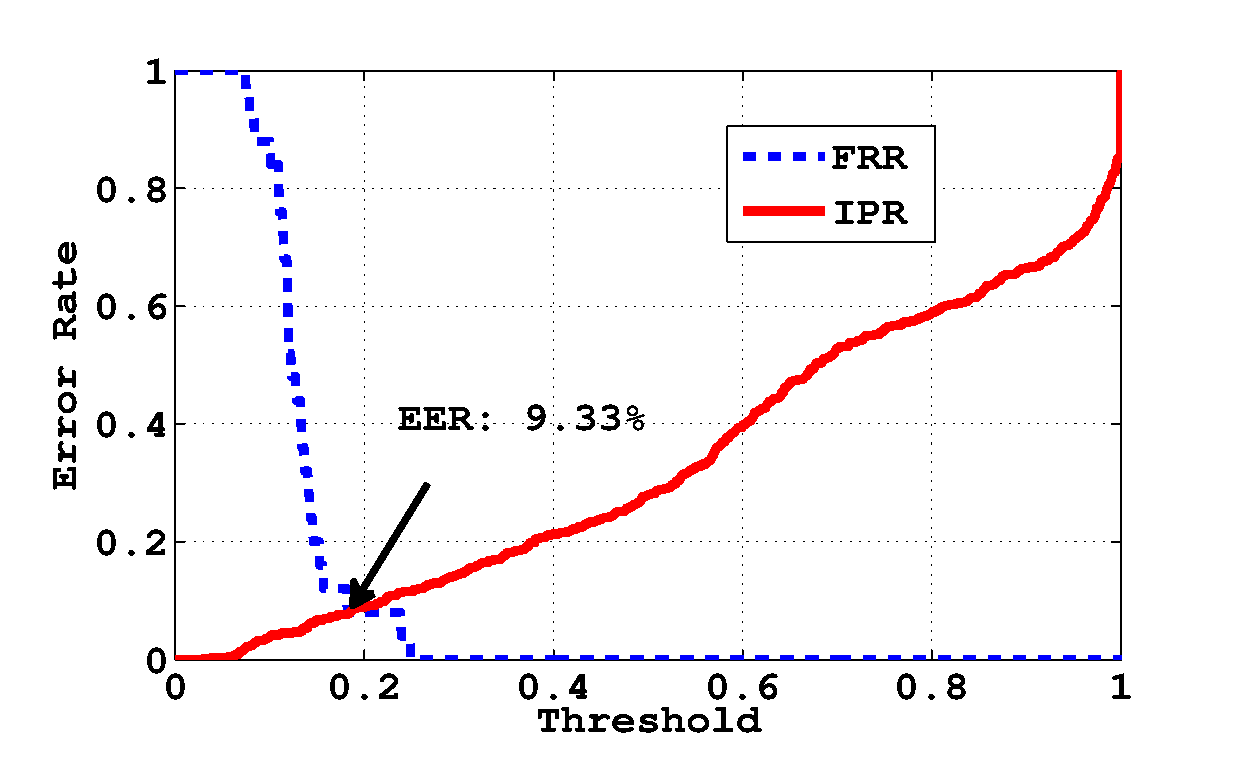
\includegraphics[width=.8\linewidth]{19M}
  \caption{Single Click R = 30ms Double Click R = 190m\\ M-Value = 1.9}
  \label{fig:sfig4}
\end{subfigure}
\caption{Plots of the False Rejection Rate and the False Acceptance Rate for four different parameter settings. The point at which the FRR and FAR intersect is the Equal Error Rate. }
\label{fig:fig}
\end{figure*}

\begin{figure*}[b!]
\begin{subfigure}{.5\textwidth}
  \centering
  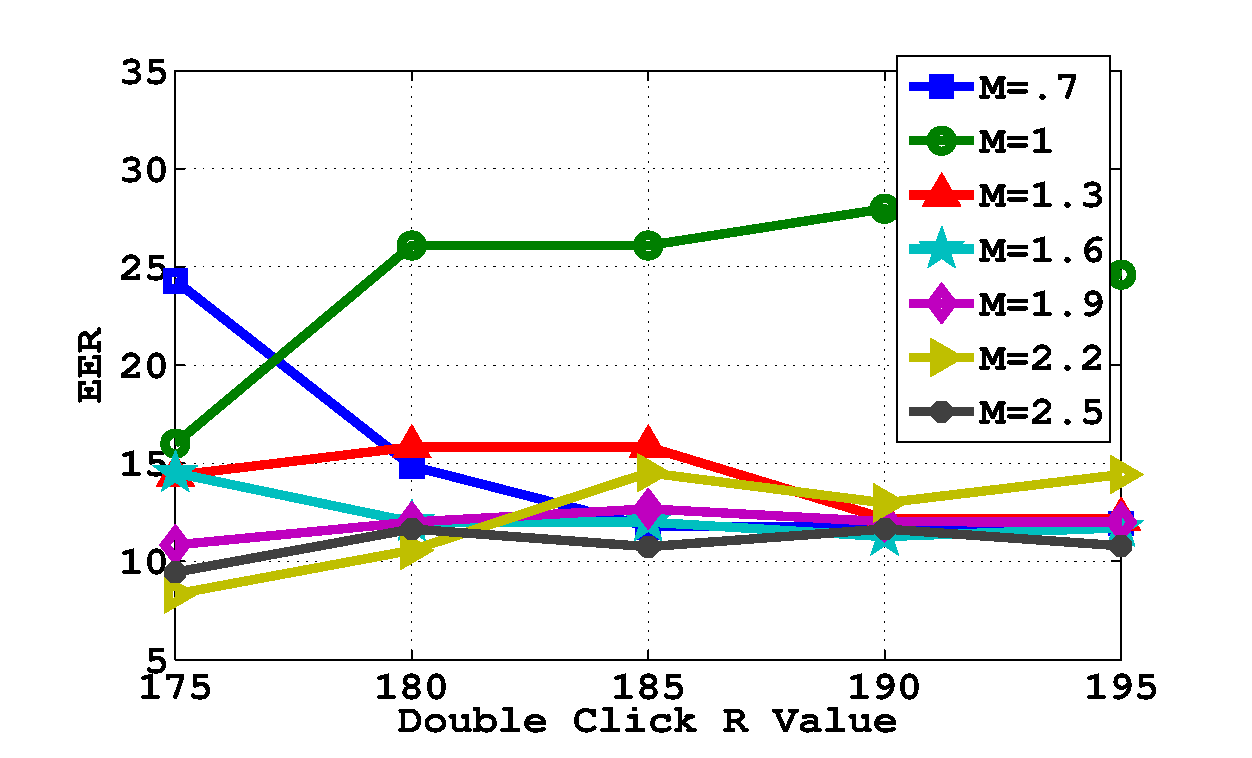
\includegraphics[width=.8\linewidth]{15.eps}
  \caption{Single Click R = 15ms \\Local Max = 24.29\% Local Min = 8.33\% \\Local Average = 14.34\% Local STD = 5.08\%}
\centering
  \label{fig:sfig1}
\end{subfigure}%
\begin{subfigure}{.5\textwidth}
  \centering
  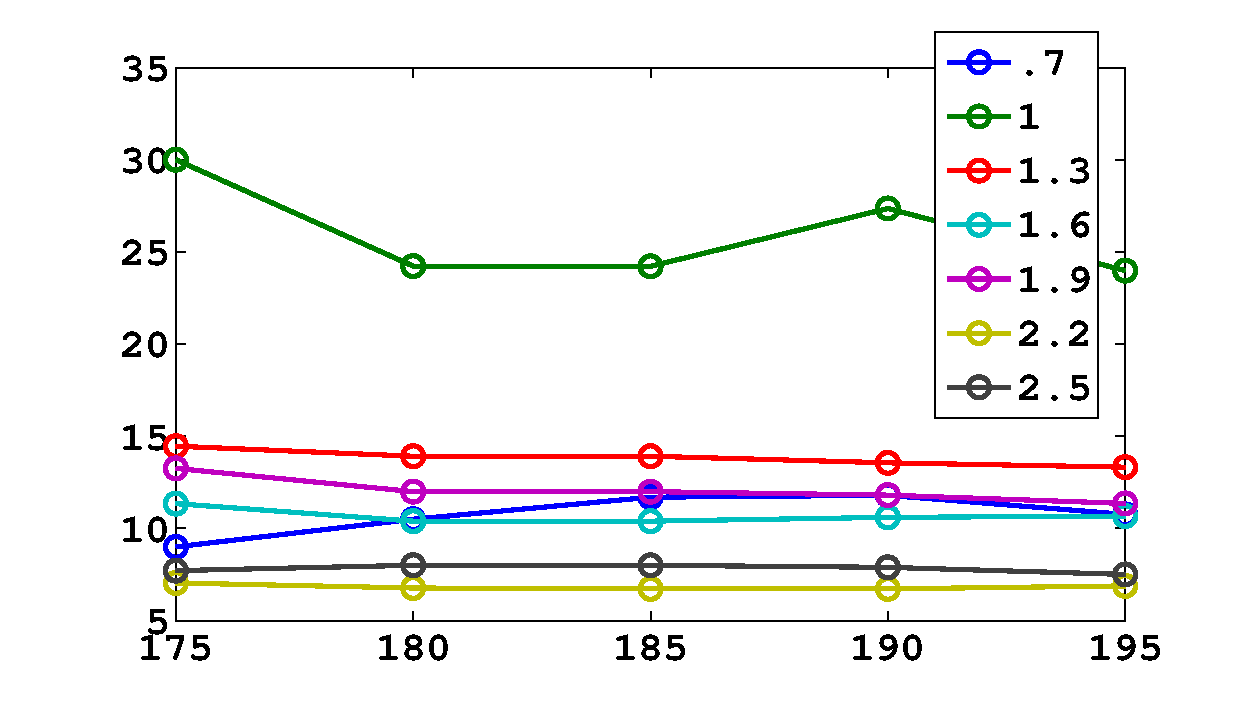
\includegraphics[width=.8\linewidth]{25.eps}
  \caption{Single Click R = 25ms \\Local Max = 30.02\% Local Min = 6.77\% \\Local Average = 12.57\% Local STD = 6.07\%}
  \label{fig:sfig2}
\end{subfigure}
\begin{subfigure}{.5\textwidth}
  \centering
  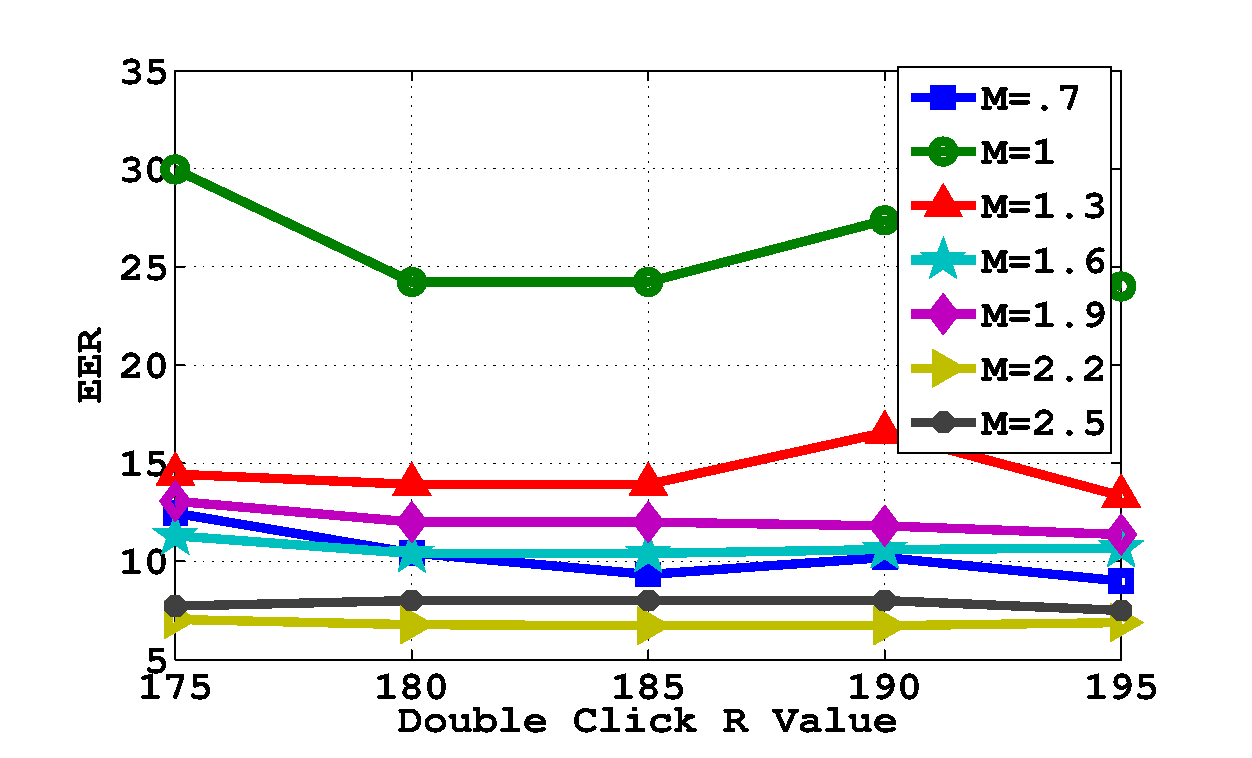
\includegraphics[width=.8\linewidth]{30.eps}
  \caption{Single Click R = 30ms \\Local Max = 29.96\% Local Min = 6.72\% \\Local Average = 12.58\% Local STD = 6.13\%}
  \label{fig:sfig3}
\end{subfigure}%
\begin{subfigure}{.5\textwidth}
  \centering
  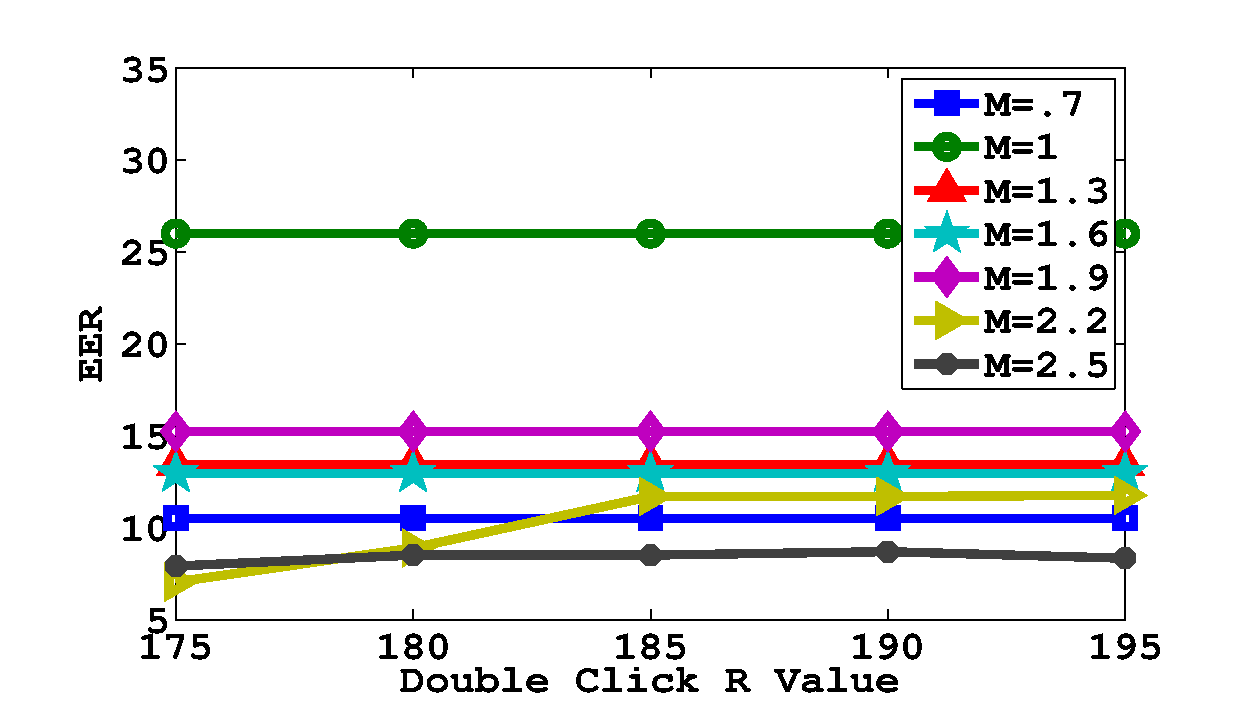
\includegraphics[width=.8\linewidth]{35.eps}
  \caption{Single Click R = 35ms \\Local Max = 26\% Local Min = 7.04\%\\Local Average = 13.82\% Local STD = 5.54\%}
  \label{fig:sfig4}
\end{subfigure}
\caption{Scatter plots of EER over the ranges of the parameter values we chose. The X-axis is Double Click R-Values, the Y-axis is the EER. Each plot is a separate Single Click R value. \\Global Max = 30.02\% Global Min = 6.72\% Global Average = 13.19\% Global STD = 5.77\%}
\label{fig:fig}
\end{figure*}


\section{Conclusion}

\section*{Acknowledgment}
We acknowledge the acknowledged acknowledgees.

\bibliographystyle{IEEEtran}

\end{document}